\claude{
\section{Theory, implementation, and experimental details}\label{app:theory}
\subsection{Dimension preservation under delay reconstruction}
The dimension interpretation has two steps. First, delay-embedding theorems give conditions under which a generic scalar observable can reconstruct the state of a deterministic system. Second, a local dimension estimator approximates the geometry of that reconstruction from finite data. The reconstruction theorem alone does not guarantee accurate estimation; the estimator alone does not establish an embedding.

For a stationary ergodic trajectory, the occupation measure can be written as $\mu(A)=\lim_{N\to\infty}N^{-1}\sum_{t=1}^{N}\mathbf{1}\{s_t\in A\}$ on sets whose boundary has zero measure. It records long-run occupancy, rather than the dimension of a finite list of observations. In Eq.~\eqref{eq:active}, $\epsilon\to0^+$ and $\epsilon\downarrow0$ denote the same right-hand limit. We use the former to emphasize that $\epsilon$ is a positive distance scale, distinct from embedding dimension $E$. Nonstationary training need not have such a limiting measure; the applied experiments therefore use finite-window scores and external reference outcomes.


\begin{proposition}[Bi-Lipschitz invariance]
Let $\mu$ have local dimension $d$ at $s$, and let $F$ be bi-Lipschitz on its support, with constants $0<c\le C<\infty$. Then the pushforward $F_\#\mu$ has local dimension $d$ at $F(s)$.
\end{proposition}
\begin{proof}
For sufficiently small $\epsilon$, the inverse image of $B(F(s),\epsilon)$ is bounded on the support between $B(s,\epsilon/C)$ and $B(s,\epsilon/c)$. Their probabilities bound the pushforward probability. The logarithms of $c$ and $C$ contribute vanishing constants after division by $\log\epsilon$, so both bounds have the same limiting exponent $d$.
\end{proof}
This property explains why bounded distance distortion preserves local dimension. A smooth embedding of a compact smooth manifold provides the needed local regularity. For a fractal support, an injective map alone need not provide the required bounds on distance distortion. The forced-system results of \citet{stark1999delay,stark2003delay} impose additional conditions and include fibre-wise formulations. Their application to a stochastic optimizer would require checking those conditions; it does not follow from observing a scalar training log.


\subsection{Recurrent, transient, and stochastic regimes}
Figure~\ref{fig:regimes} makes the assumptions operational. A recurrent trajectory returns to nearby states, a transient moves through a region without repeated visits, and stochastic forcing fills the observed space according to the noise and the observation channel. The same numerical estimator returns a value in all three cases; the regime determines whether that value can be called a dimension.

\begin{figure}[H]
\centering
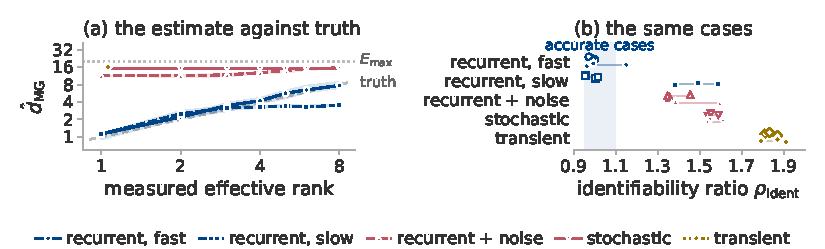
\includegraphics[width=.92\linewidth]{figures/icomp_regimes.pdf}
\caption{\claude{Regime diagnostics from the synthetic study. The left panel compares MG with an independently measured effective rank; the right panel separates recurrent and non-recurrent records using identifiability. The shaded region marks the tested regime in which the component interpretation is supported.}}
\label{fig:regimes}
\end{figure}

\begin{figure}[H]
\centering
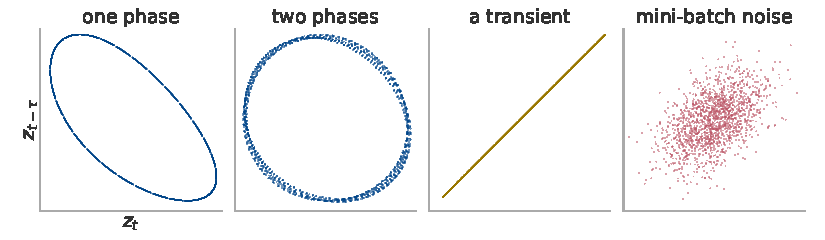
\includegraphics[width=.86\linewidth]{figures/icomp_shapes.pdf}
\caption{\claude{Delay reconstructions of four cases. A recurrent one-phase signal closes a loop; two phases fill a higher-dimensional set; a transient follows a path without returning; stochastic forcing fills the available region. These pictures explain why recurrence and identifiability are required before reading MG as active dimension.}}
\label{fig:shapes}
\end{figure}

\begin{figure}[H]
\centering
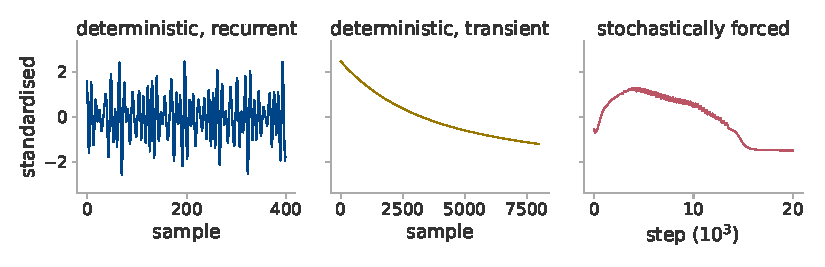
\includegraphics[width=.86\linewidth]{figures/icomp_traces.pdf}
\caption{\claude{The same scalar-log viewpoint across regimes: recurrent forcing, a transient optimization path, and a stochastically forced training record. The estimator is applied to all three, while the interpretation changes with the regime.}}
\label{fig:traces}
\end{figure}

\subsection{Computing the pooled estimator}
For reproducibility, the implementation can be summarized as follows. The dither and numerical floors only handle ties and degeneracy; they do not provide a statistical correction. The implementation standardizes first, adds Gaussian dither with scale $10^{-9}$, floors distances at $10^{-8}$ and local sums at $10^{-5}$, and marks a window when more than 1\% of either quantity reaches a floor.

\begin{center}
\fbox{\begin{minipage}{0.96\linewidth}\small
\textbf{Input:} scalar record $x_{1:N}$, lag $\tau$, embedding dimension $E$, number of neighbors $k$, Theiler exclusion $T$.

1. Reject nonfinite, constant, or too-short records. Standardize $x_t$ and add fixed-scale dither, giving $z_t$.\\
2. Form $y_t=(z_t,z_{t+\tau},\ldots,z_{t+(E-1)\tau})$.\\
3. For each $y_i$, find the $k$ closest $y_j$ with $|i-j|>T$. Return an unavailable estimate if neighbors are insufficient.\\
4. Accumulate $S_i=\sum_{j=1}^{k-1}\log(r_{ik}/r_{ij})$, recording distance and sum floors.\\
5. Set $n=N-(E-1)\tau$, the number of valid delay vectors. Return $\widehat d_{\rm MG}=(n(k-1)-1)/\sum_{i=1}^{n} S_i$ and the degeneracy flags.
\end{minipage}}
\end{center}

The change detector is separate from the estimator: it compares recent and earlier blocks of window estimates. This separation lets us compare MG with other scalar features under the same causal decision rule.

\subsection{Affine invariance and its implementation boundary}
\begin{proposition}[Affine invariance of the ideal scalar estimate]
For a finite nonconstant record, fixed delay and neighbor settings, and no numerical dither, the MG formula is unchanged by replacing every observation with $ax_t+b$, for any $a\ne0$, provided the estimate is defined.
\end{proposition}
\begin{proof}
After centering and dividing by standard deviation, the transformed series is the original standardized series multiplied by $\operatorname{sign}(a)$. All pairwise Euclidean distances of its delay vectors are identical. Temporal exclusions and admissible neighbors therefore remain unchanged, as do all distance ratios and their pooled estimate.
\end{proof}
The implemented code adds Gaussian dither of scale $10^{-9}$ after standardization, floors distances at $10^{-8}$ and local log-ratio sums at $10^{-5}$, and records the fractions affected by these floors. Positive affine changes preserve the standardized input in exact arithmetic and preserve a run with the same dither. A negative rescaling preserves the distribution under symmetric dither, but need not give exactly equal values with the same realized dither. Finite precision and almost-constant records require separate checks. The proposition concerns a whole-window affine transformation: a scale change within a window is a different time series.

\subsection{Pooling and dependence}
The numerator $n(k-1)-1$ is the bias correction used by the existing implementation. Its Gamma-model motivation assumes idealized independent local statistics. Neighbor reuse and serial dependence mean that this correction is not a general finite-sample unbiasedness guarantee for the records in this paper. We use the same implementation throughout, preserve degeneracy flags, and do not clip large estimates to $E$. The Theiler exclusion removes temporally adjacent candidates but does not make the remaining observations independent.

\section{Configurations and reproducibility}\label{app:settings}
Tables and figures are generated from saved CSV/JSON experimental outputs. The accompanying source bundle records file hashes and maps numerical claims to their sources. We specify the observable, estimator settings, and development/test split for each task. All tasks use the same estimator; window length and lag are chosen for the relevant timescale.

\begin{table*}[t]
\centering\small
\caption{\claude{Primary configurations. An exclusion of ``span'' is $(E-1)\tau$. The adaptive generator lag is one quarter of the autocorrelation time, capped so the delay span occupies at most one eighth of the window; its exclusion is capped at 320. Alternative settings are reported as sensitivity checks, not substituted for the primary results.}}
\begin{tabular}{llrrrrll}
\toprule
Experiment & Observable & $W$ & $E$ & $\tau$ & $k$ & Theiler exclusion & Stride \\
\midrule
Digits head & state-based & 8,000 & 20 & 4 & 20 & span; cap 150 & 3,000 \\
Regression & loss / probe & 2,048; 8,192 & 16 & 1 & 10 & 100 & endpoints \\
Generator & neuron zero & 8,192 & 20 & adaptive & 20 & ACF; cap 320 & 8,192 \\
CNN / ResNet-18 & parameter norm & 1,000 & 20 & 1 & 20 & span & 500 \\
VAE & probe NLL & 512 & 20 & 1 & 20 & 39 & 128 \\
Walker2d & joint / action scalar & 2,048 & 20 & 8 & 20 & 312 & 512 / 1,024 \\
\bottomrule
\end{tabular}
\end{table*}

\paragraph{Exact adaptive rules.}
For centered samples $z_t$, define $a(\ell)=\sum_{t=1}^{W-\ell}z_tz_{t+\ell}/\sum_{t=1}^Wz_t^2$. The autocorrelation time $t_a$ is the first lag with $a(\ell)<e^{-1}$, or $W$ if none exists. The adaptive generator uses
\[
\begin{aligned}
\tau_0&=\max(1,\operatorname{round}(t_a/4)),\\
\tau&=\min\{\tau_0,\max(1,\lfloor W/[8(E-1)]\rfloor)\}.
\end{aligned}
\]
The implementation uses nearest-even rounding. Theiler settings resolve to $T=\min(T_{\max},T_0)$, where $T_0=(E-1)\tau$ for the embedding rule and $T_0=\max((E-1)\tau,t_a)$ for the autocorrelation rule. An explicit integer is also capped. Thus a cap can shorten the requested exclusion below the embedding span; report both the rule and its resolved value. The primary digits configuration uses the embedding rule (76 samples), not an uncapped autocorrelation rule.

The historical digits sweep uses stride 3,000 on the 26,000 post-burn samples ($\max(500,\lfloor(N-W)/6\rfloor)$); development used stride 2,000. The known-mode table uses endpoint windows; its additional switch trace uses $W=4,096$ and stride 2,048. Walker uses stride 512 in the early repair series and 1,024 in later three-window summaries. Generator windows are disjoint. The cyclic VAE uses stride 64. These variations are fixed for each procedure, not selected after comparing outcomes.

\paragraph{Window length and recurrence requirements.}
A window must leave enough admissible neighbors after delay reconstruction and temporal exclusion. Meeting the software minimum is necessary but does not guarantee an accurate estimate. For dimension estimation, the window should contain repeated visits within one regime. The lag must also expose the phase structure: increasing record length cannot compensate for delay vectors that cover only a nearly linear segment. For detection, longer windows stabilize estimates but blur transitions. We report detection delay to make this tradeoff explicit.

\paragraph{Units of replication.}
The CNN interventions share seeds and pre-intervention histories; rescaling and smoothing are transformations of unchanged logs. Generator tasks reuse initialization seeds. The VAE branches share initial trajectories, data, and probes. The Walker continuations share a learned starting policy. We report detection totals and paired contrasts at these levels; we do not treat overlapping windows or transformed logs as independent draws from a population. The VAE intervals are percentile bootstrap intervals over nine paired confirmation seeds, using 20,000 resamples and bootstrap seed 20260929. They measure initialization/batch variation conditional on the selected data and observable.

\section{Development systems and MLP-based recovery}\label{app:controlled}
\subsection{Analytic and driven-learning evaluation}
The synthetic suite includes an analytic matrix with independent oscillatory entries and learning systems with time-dependent targets or forcing: online regression, logistic regression, a frozen nonlinear decoder, and an MLP in a parameter subspace. To distinguish input variation from learned motion, we set the learning rate to zero and check whether each observable still changes. Several early loss and gradient observables continue varying. Their dimension estimates can recover the forcing structure, but cannot be attributed solely to changing parameters. The digits-head experiment below addresses this ambiguity with state-based observables that become constant when learning stops.

\begin{table}[h]
\centering\small
\caption{\claude{Synthetic results against the specified references. Mean absolute error (MAE) averages rank--seed--observable combinations. The driven-target MLP signal still varies with frozen parameters; its error describes the driven signal, not parameter motion alone.}}
\begin{tabular}{lrr}
\toprule
Construction & Range & MAE \\
\midrule
Analytic oscillating matrix & 1--8 & 0.27 \\
Driven-target MLP subspace & 1--20 & 0.92 \\
Digits head, covariance reference & 1--8 & 0.90 \\
\bottomrule
\end{tabular}
\end{table}

In the digits experiment, we train and freeze an MLP feature extractor, then train a linear head in a fixed affine parameter subspace. The cross-entropy loss assigns weights to twelve fixed data groups. For the historical digits experiment, weights are $w_i(t)=\max\{0.05,1+0.8\sum_{j=1}^r G_{ji}\sum_{\ell=1}^r A_{j\ell}\sin(2\pi f_\ell t+\phi_\ell)\}$. Here $G$ identifies the twelve fixed data groups and $A$ equalizes their linearized forcing directions and gains. For $r>1$, $f_j=2^{a_j}/16$, with $a_j=0.03+0.94(b_j-\min b)/(\max b-\min b)$ and $b_j=\operatorname{frac}(\sqrt{p_j})$ for the first $r$ primes; for $r=1$, $f_1=\sqrt2/16$. Phases are uniform on $[0,2\pi)$ from NumPy's generator seeded by $31+\text{seed}$; group assignment uses $7717+\text{seed}$. The drive amplitude is 0.8 and the preconditioned head step is 0.15. These describe the archived implementation behind the reported scores; the newer code organizes random streams differently. Development uses seeds 90--92 and ranks 2,4,6; evaluation uses seeds 0--3 and held-out ranks 1,3,5,8. The selected settings are $E=20$, $\tau=4$, $k=20$, and an 8,000-point window. This configuration lies on the boundary of the search grid and is held fixed for evaluation; the search does not establish a global optimum.

All usable state-based observables order the held-out ranks correctly. The mean error against measured covariance effective rank is 0.90 across individual records; aggregating by rank before computing the error gives 0.382. We report the former because these aggregations answer different questions. Errors by observable are 0.60 for fixed-probe loss, 0.41 for parameter norm, 0.34 for a fixed parameter projection, and 1.81 for gradient norm. Instantaneous mini-batch loss continues varying with frozen parameters, while quantized probe accuracy is degenerate; neither supports the parameter-dimension interpretation. The specified phases define the intended structure, and the covariance reference checks which directions are measurably excited.

\subsection{Dense regression with endogenous modes}
The data matrix has 256 rows and 32 columns, full column rank, and Hessian $H=X^\top X/256$. Orthogonal rotations make the data and learned weights dense. Eigenvalues are grouped into $r$ repeated values, with a single excited direction within each group. For heavy-ball momentum one and step size one, the error in group $j$ obeys
\[
q_{j,t+1}=2\cos(\omega_j)q_{j,t}-q_{j,t-1},
\qquad \lambda_j=2(1-\cos\omega_j).
\]
The selected irrational frequencies produce $r$ independent phases. All 32 original coordinates move. Three seeds vary bases, teacher directions, and probes, but the normalized training-loss dynamics are identical up to rounding for a fixed spectrum. These are coordinate/observer checks rather than three independent loss processes.

\begin{table}[h]
\centering\small
\caption{\claude{Known-mode regression: median scalar MG. Settings are fixed across $r$. A longer record does not uniformly reduce bias.}}
\begin{tabular}{rrrr}
\toprule
$r$ & Loss, 2,048 & Loss, 8,192 & Probe, 8,192 \\
\midrule
1 & 0.90 & 1.12 & 1.01 \\
2 & 2.39 & 2.57 & 2.55 \\
4 & 3.71 & 4.99 & 4.11 \\
6 & 5.88 & 7.00 & 4.98 \\
\bottomrule
\end{tabular}

\end{table}

Selective damping sets momentum to 0.98 in two of four groups at step 8,192. The comparison uses disjoint 8,192-point windows before damping and after the transition, with the latter starting at 12,288. Across three seeds, loss-based MG changes from 4.97 to 2.56 in every run; the median probe estimate changes from 4.15 to 2.63. The corresponding loss values are deterministic up to the tested seed changes in coordinates and probes, so the table reports the three-run range rather than treating the repeated loss curves as independent trajectories. With ordinary momentum 0.99 on all groups, learning converges and late losses reach rounding scale. Standardization can then produce spurious high estimates; the absolute pre-standardization scale must be checked.

\begin{table}[h]
\centering\small
\caption{\claude{Three-seed variation in the selective-damping regression experiment.}}
\label{tab:regression_variation}
\begin{tabular}{lrrrr}
\toprule
Signal & Phase & Median & Minimum & Maximum \\
\midrule
loss & before & 4.971432 & 4.971432 & 4.971432 \\
loss & after & 2.562791 & 2.562791 & 2.562791 \\
probe error & before & 4.153513 & 3.601192 & 4.206165 \\
probe error & after & 2.634185 & 1.995991 & 2.680959 \\
\bottomrule
\end{tabular}

\end{table}

\subsection{Learned autonomous generators}
The 1,000-unit generator evolves as
\[
\begin{aligned}
\boldsymbol h_{t+1}&=0.9\boldsymbol h_t+
0.1(J\tanh\boldsymbol h_t+U\boldsymbol z_t),\\
\boldsymbol z_t&=A^\top\tanh\boldsymbol h_t.
\end{aligned}
\]
Here $\boldsymbol h_t$ is the network state, $J$ the recurrent matrix with gain 1.2, $U$ the output-feedback matrix, and $A$ the readout trained by FORCE/RLS for 100,000 simulation steps. Frequencies are proportional to $1,\sqrt2,\sqrt3,\sqrt5$ for T1--T4; H2/H4 use integer harmonics, and M4 uses $1,2,\sqrt2,2\sqrt2$. All seven tasks use seeds 1--5. After training, we discard 5,000 burn-in steps and record 32,768 autonomous samples. The reported MG value is the median over four disjoint 8,192-point windows on neuron zero. Neurons one and two provide fixed robustness checks.

The Lyapunov reference uses twelve tangent vectors and a near-zero threshold of $-0.02$ chosen in advance. The number of near-zero exponents agrees with the target phase dimension in 31/35 cases. H2 has weakly contracting directions near the threshold and is overestimated in four seeds. Thus even this reference has finite-time ambiguity. MG has finite-resolution error as well: one periodic H2 record gives 0.73, T2 has median 2.84, and T3/T4 overlap. The reliable comparison is the distinction between phase structures, especially in the harmonic references; exact recovery across $d=1$--$4$ is not established.

As a robustness check, we re-evaluated the stored H4, M4, and T4 generators on three neurons, two windows, and three additive-noise levels. On neuron zero, MG preserved the expected H4 $<$ M4 $<$ T4 ordering on all five seeds for 4,096 samples with no added noise and with noise of standard deviation $0.01$ times the signal standard deviation. At noise level $0.05$, the ordering held on two of five seeds for the shorter window and on none for the longer window. The corresponding median estimates were $(1.14,4.56,6.30)$ in the clean short-window condition and $(5.53,5.12,6.75)$ in the noisy short-window condition. This stress test supports robustness to small observation noise, while making the breakdown at larger noise explicit.

For the separate 256-unit motion experiment, gain is 1.5 and FORCE learns a figure-eight target for 40,000 simulation steps. Each frozen checkpoint is evaluated after 2,000 burn-in steps over 8,192 recorded states. The chaotic initializations comprise the first five eligible seeds among sequential candidates 6--30, selected by a positive pretraining Lyapunov criterion; thirteen candidates were examined, yielding seeds 7,9,15,16,18. No MG value enters selection. The unselected initial seeds 1--5 are retained separately because some start nonchaotic. This is conditional evidence for learning from chaos, not an estimate of how often random networks become chaotic or learn a stable cycle.

\section{Applied training procedures and full comparisons}\label{app:applied}
\subsection{CNN and ResNet interventions}
The small CNN has three convolutional layers with 16, 32, and 32 ReLU channels, $3\times3$ kernels, max pooling after the first two layers, adaptive average pooling, and a ten-class linear head; it has 14,666 parameters and no normalization. It uses 10,000 CIFAR-10 images, SGD step 0.02, momentum 0.9, weight decay $5\cdot10^{-4}$, and batches of 64 sampled with replacement. The graded study runs 10,000 updates with an intervention at update 4,000. The before/after summaries use windows lying within the designated pre/post intervals, excluding the immediate mixed transition.

The learning-rate interventions divide the step size by 3, 10, or 100. Freezing leaves the later layers, only the head, or only its bias trainable. Pruning masks 50\%, 80\%, or 95\% of weights. Some interventions rebuild SGD for the remaining trainable parameters, which also changes optimizer state. Their measured effect therefore includes that change and cannot be attributed to the number of parameters alone. Increased-batch references multiply batch size by four. Rescaling multiplies the base log by ten after update 4,000. Smoothing replaces that suffix by the causal 16-sample moving average $\bar x_t=\sum_{j=0}^{15}x_{t-j}/16$, using the preceding original samples at the boundary; neither transformation retrains the network.

The CNN IAAFT comparison uses two surrogates per window and reports their median MG, with RNG seed equal to the window start. Each surrogate uses 100 alternating spectrum/rank projections. Endpoint matching can trim up to 15\% of the window before randomization, so spectrum and marginal preservation refer to the retained segment; it is a descriptive reference, not a matched-length significance test.

\begin{table*}[t]
\centering\small
\caption{\claude{CNN interventions at all tested strengths, on four held-out seeds. Changes are medians of paired record ratios. Update covariance and the fraction of moving parameters provide independent comparisons. Stronger pruning does not always produce a larger MG decline.}}
\begin{tabular}{lrrrrr}
\toprule
Intervention & MG before & MG after & MG change & Update PR change & Moving parameters \\
\midrule
No intervention & 4.31 & 4.32 & +0.4\% & +40.3\% & 100.00\% \\
Batch $\times4$ & 4.31 & 4.85 & +12.8\% & -7.3\% & 100.00\% \\
Log $\times10$ & 4.31 & 4.32 & +0.4\% & +40.3\% & 100.00\% \\
Smoothed log & 4.31 & 4.44 & +3.3\% & +40.3\% & 100.00\% \\
Step / 3 & 4.31 & 4.35 & +0.9\% & -5.4\% & 100.00\% \\
Step / 10 & 4.31 & 3.95 & -8.3\% & -21.6\% & 100.00\% \\
Step / 100 & 4.31 & 3.85 & -11.5\% & -20.9\% & 100.00\% \\
Freeze first two convolutions & 4.31 & 4.27 & -1.8\% & -13.6\% & 65.31\% \\
Train head only & 4.31 & 3.51 & -18.5\% & -43.5\% & 2.25\% \\
Train head bias only & 4.31 & 3.58 & -16.7\% & -68.4\% & 0.07\% \\
Prune 50\% & 4.31 & 3.80 & -12.7\% & +14.7\% & 50.30\% \\
Prune 80\% & 4.31 & 3.59 & -17.5\% & -10.3\% & 20.48\% \\
Prune 95\% & 4.31 & 3.79 & -11.5\% & -45.3\% & 5.55\% \\
\bottomrule
\end{tabular}

\end{table*}

Detector development searches $M\in\{2,3,4\}$ and $B\in\{3,4,6\}$. For each pair, its drop threshold is the smallest giving no false positives on development nulls, plus a margin of 0.02. The selected pair maximizes development event detection, with shorter delay as a tie breaker. Companion-statistic directions are chosen on development data as well. The rule is frozen for the new graded seeds and for ResNet. The selected MG threshold is 0.0882988401. The primary 27/28 result covers seven strong intervention types on four seeds; weak types are reported separately. The 16 references comprise base, increased batch, rescaled base, and smoothed base on the same four seeds. Thus these totals describe a matched benchmark rather than independent Bernoulli trials.

\subsection{Natural scalar baselines}\label{app:baselines}
We computed additional scalar features on the same saved parameter-norm records. Permutation entropy measures the diversity of local ordinal patterns~\citep{bandt2002permutation}; sample entropy measures the recurrence of similar short templates~\citep{richman2000physiological}; normalized increments measure local motion; and spectral entropy summarizes the detrended periodogram. We also tested a one-sided Page CUSUM~\citep{page1954continuous} on each window feature. Every feature used the same event definition, development seeds, detector family, and held-out seeds as MG. These comparisons test complementarity, not population-level superiority.

\begin{table}[h]
\centering\small
\caption{\claude{Natural scalar features on the held-out CNN benchmark. Each detector is fixed on the earlier seeds. Successful detections cover seven strong intervention types across four seeds; false positives cover four reference types across four seeds.}}
\label{tab:extra_baselines}
\scriptsize\setlength{\tabcolsep}{2pt}
\begin{tabular}{lrrr}
\toprule
Feature & Hits & False positives & Median delay \\
\midrule
MG & 27/28 & 0/16 & 1,000 \\
Abs. increments & 27/28 & 0/16 & 500 \\
Norm. increments & 28/28 & 0/16 & 1,500 \\
Perm. entropy & 28/28 & 7/16 & 1,500 \\
Sample entropy & 28/28 & 4/16 & 1,500 \\
Spectral entropy & 4/28 & 2/16 & 2,750 \\
Trend crossings & 15/28 & 5/16 & 1,000 \\
Lag-one corr. & 0/28 & 0/16 & --- \\
Detrended std. & 28/28 & 10/16 & 500 \\
Level & 4/28 & 0/16 & 1,000 \\
\bottomrule
\end{tabular}
\end{table}

\begin{table}[h]
\centering\small
\caption{\claude{False positives by type for the block detector. The reference records share the four held-out seeds; the table therefore describes this matched benchmark rather than independent false-positive probabilities.}}
\label{tab:baseline_references}
\scriptsize\setlength{\tabcolsep}{2pt}
\begin{tabular}{lrrrr}
\toprule
Feature & Base & Batch $\times4$ & Rescaled & Smoothed \\
\midrule
MG & 0 & 0 & 0 & 0 \\
Abs. increments & 0 & 0 & 0 & 0 \\
Norm. increments & 0 & 0 & 0 & 0 \\
Perm. entropy & 3 & 0 & 3 & 1 \\
Sample entropy & 1 & 0 & 1 & 2 \\
Spectral entropy & 0 & 2 & 0 & 0 \\
Trend crossings & 1 & 2 & 1 & 1 \\
Lag-one corr. & 0 & 0 & 0 & 0 \\
Detrended std. & 2 & 2 & 4 & 2 \\
Level & 0 & 0 & 0 & 0 \\
\bottomrule
\end{tabular}
\end{table}

The primary block detector uses $W=1,000$, stride 500, and excludes feature windows ending at or before update 1,500 from the detection history. MG uses $M=2$, $B=3$, and a drop threshold of $0.08829884$; each baseline selects its direction and threshold on the development records. Permutation entropy uses ordinal order five, unit delay, stable sorting for ties, and normalization by $\log(5!)$; sample entropy uses template length two, unit delay, Chebyshev distance, tolerance $0.2$ times the window standard deviation, and self-match exclusion; normalized increments divide mean absolute increments by the window standard deviation; spectral entropy uses the normalized detrended periodogram; trend crossings count sign changes after linear detrending. Page CUSUM uses the same features, a past-only warm-up, drift selected from $\{0.25,0.5,1\}$, and the parameters in Table~\ref{tab:baseline_rules}. The block score is $s(1-\operatorname{median}_{M}/\operatorname{median}_{B})$, with direction $s\in\{-1,1\}$; MG fixes $s=1$. Development searches $M\in\{2,3,4\}$, $B\in\{3,4,6\}$. Its threshold exceeds the largest reference score by 0.02, and selection maximizes event detections, then minimizes median delay. A baseline ratio is skipped when the reference magnitude is at most $10^{-12}$.

CUSUM fixes its mean $\mu_0$ and scale $\sigma_0=\max(\operatorname{std}_0,0.01|\mu_0|,10^{-10})$ from feature windows ending at 2,000--3,500. Starting at zero, $C_j=\max\{0,C_{j-1}+s(\mu_0-v_j)/\sigma_0-\kappa\}$; a detection occurs when $C_j>h$. Both directions and the stated drift grid are fixed, with $h$ exceeding the largest development-reference score by 0.5. These rules are causal but warm-up must finish before scoring; they are not detectors available from the first training step.

\begin{table*}[t]
\centering\small
\caption{\claude{Selected detector parameters. The block sign is listed; all selected CUSUM signs are recorded in \texttt{new\_results/rules.json}. Full-precision values in that file define the implemented thresholds.}}
\label{tab:baseline_rules}
\begin{tabular}{lrrrrrr}
\toprule
Feature & $M$ & $B$ & Sign & $\delta$ & CUSUM drift & CUSUM $h$ \\
\midrule
MG & 2 & 3 & 1 & 0.0882988 & 0.25 & 44.3109 \\
Abs. increments & 2 & 3 & 1 & 0.338305 & 1.0 & 19.7929 \\
Norm. increments & 4 & 4 & -1 & 0.0289438 & 0.25 & 5.90329 \\
Perm. entropy & 2 & 6 & -1 & 0.339038 & 1.0 & 7.79449 \\
Sample entropy & 2 & 3 & -1 & 0.186699 & 0.25 & 9.86063 \\
Spectral entropy & 3 & 3 & -1 & 1.29961 & 0.25 & 6.74364 \\
Trend crossings & 2 & 4 & 1 & 0.662857 & 0.5 & 2.31626 \\
Lag-one corr. & 2 & 3 & 1 & 0.0238814 & 0.25 & 0.653369 \\
Detrended std. & 2 & 3 & -1 & 0.305439 & 0.25 & 0.5 \\
Level & 2 & 3 & 1 & 0.02 & 0.25 & 0.5 \\
\bottomrule
\end{tabular}

\end{table*}

\begin{table}[h]
\centering\scriptsize\setlength{\tabcolsep}{2pt}
\caption{\claude{Past-only CUSUM on the held-out CNN records. Thresholds are selected on development records; the table reports strong-event detections, reference false positives, and median delay.}}
\label{tab:cusum}
\begin{tabular}{lrrr}
\toprule
Feature & Detected & FP & Delay \\
\midrule
MG & 17/28 & 0/16 & 3,500 \\
Abs. increments & 27/28 & 12/16 & 2,500 \\
Norm. increments & 28/28 & 4/16 & 1,000 \\
Perm. entropy & 28/28 & 4/16 & 1,000 \\
Sample entropy & 28/28 & 4/16 & 1,250 \\
Spectral entropy & 5/28 & 1/16 & 500 \\
Trend crossings & 13/28 & 3/16 & 1,000 \\
Lag-one corr. & 1/28 & 0/16 & 500 \\
Detrended std. & 28/28 & 4/16 & 500 \\
Level & 0/28 & 0/16 & --- \\
\bottomrule
\end{tabular}

\end{table}

On this benchmark, normalized increments detect 28/28 events with 0/16 reference false positives, compared with 27/28 and 0/16 for MG. Absolute increments match MG in detections and false positives with shorter median delay. Both entropy features detect all events but produce reference false positives. Simple features achieve higher detection rates in this CNN benchmark. MG provides a geometric statistic that is also evaluated on the specified generator, VAE, RL, and full-state timing benchmarks.

We evaluated ten additional seeds using a fixed procedure and historical detector rules fixed before training. This transfer test produced 19/30 intervention detections for MG; five of ten ordinary-training references contained threshold crossings, and six intervention branches had crossings before the assigned intervention time. Mean absolute increments produced 30/30 detections with no reference false positives. Normalized increments produced 29/30 detections and false positives in two of ten references. This confirmation indicates that the original CNN benchmark supports the fixed comparison above, but its detector threshold does not transfer universally across initialization and event schedules.

\begin{table*}[t]
\centering\small
\caption{\claude{Post-hoc horizon sensitivity with thresholds and first detections unchanged. Entries are detections within the specified number of updates; FP uses each complete reference record and is independent of the event horizon.}}
\label{tab:horizons}
\begin{tabular}{lrrrrr}
\toprule
Feature & 500 & 1,000 & 2,000 & 5,000 & FP \\
\midrule
MG & 8/28 & 16/28 & 22/28 & 27/28 & 0/16 \\
Abs. increments & 15/28 & 16/28 & 26/28 & 27/28 & 0/16 \\
Norm. increments & 0/28 & 0/28 & 21/28 & 28/28 & 0/16 \\
Perm. entropy & 0/28 & 0/28 & 23/28 & 28/28 & 7/16 \\
Sample entropy & 8/28 & 13/28 & 27/28 & 28/28 & 4/16 \\
Spectral entropy & 0/28 & 0/28 & 0/28 & 4/28 & 2/16 \\
Trend crossings & 0/28 & 15/28 & 15/28 & 15/28 & 5/16 \\
Lag-one corr. & 0/28 & 0/28 & 0/28 & 0/28 & 0/16 \\
Detrended std. & 25/28 & 27/28 & 27/28 & 28/28 & 10/16 \\
Level & 0/28 & 4/28 & 4/28 & 4/28 & 0/16 \\
\bottomrule
\end{tabular}

\end{table*}
The MG horizon sensitivity on the original held-out records (Table~\ref{tab:horizons}) is 8/28, 16/28, 22/28, and 27/28 detections at horizons 500, 1,000, 2,000, and 5,000 updates, respectively; reference false positives remain 0/16 at all four horizons.

ResNet-18 runs use the full CIFAR-10 training set, new seeds 20--22, and scratch/pretrained settings. SGD uses momentum 0.9, weight decay $5\cdot10^{-4}$, initial step 0.02, and batch 128 without augmentation; the pretrained setting uses $64\times64$ images and ImageNet normalization. The pretrained network retains the standard $7\times7$, stride-two stem and max pool and replaces its classifier by a ten-class head. The scratch network uses a $3\times3$, stride-one stem, no initial max pool, and $32\times32$ CIFAR-normalized inputs. MG and the rule transfer unchanged. A 1,024-coordinate CountSketch of updates provides a tractable covariance reference. The head-only intervention succeeds in both settings; learning-rate and pruning detection does not. The six freezing records and 24 references reuse three seeds and two initial-model settings.

\subsection{ReLU-death stress test}
A separate experiment uses six new seeds 30--35 and abrupt learning-rate shocks, with doses chosen on a pilot using activation death and accuracy, not MG. The tested learning-rate multipliers are 20, 30, 50, and 100 for one update; 15 for three updates; and 20 for two updates, followed by restoration of the base rate. A channel is classified as dead if it is zero on all 500 diagnostic images. An event requires an increase of at least 0.05 in the fraction of dead channels. There are 42 training runs, augmented by rescaled and smoothed base logs. Twenty-three runs meet the death criterion; two catastrophic whole-network failures are excluded from the prescribed eligible-event score and remain reported separately. The 42 runs comprise seven arms on six seeds: 23 meet the event criterion and 19 do not. Removing two catastrophic events leaves 21 eligible events; six rescaled and six smoothed base logs augment the 19 non-events to 31. Thus $42-2+12=52$ scored records, not 52 independent training runs.

\begin{table}[h]
\centering\small
\caption{\claude{Boundary case: the transferred detector on ReLU death. Rules are fixed before the confirmation results.}}
\begin{tabular}{lrr}
\toprule
Statistic & Detected / 21 & False positives / 31 \\
\midrule
MG & 12 & 12 \\
Trend crossings & 19 & 7 \\
Loss stagnation & 21 & 8 \\
Detrended std. & 21 & 25 \\
Lag-one correlation & 0 & 0 \\
\bottomrule
\end{tabular}
\end{table}
MG changes are nonmonotone in channel death: moderate loss of channels and catastrophic disruption can move the estimate in opposite directions. The CNN success therefore concerns the tested sustained training interventions and is not a generic failure detector.

\subsection{Text VAE and preservation reference}
We select 6,000 training and 256 fixed evaluation sentences with seed 20260929. Each has 8--24 words before the end-of-sentence token. A 2,000-token vocabulary is built from the training data. Shared embeddings have dimension 48, both GRUs have hidden size 64, and the diagonal Gaussian latent code has dimension 16. The decoder receives the code in its initial state and at every decoding step. Training uses teacher forcing, Adam with learning rate 0.001, batch size 32, gradient-norm clipping at five, and no dropout. The loss sums reconstruction NLL within each sentence, adds $\beta$ times the KL term, and averages over sentences. Since the encoder observes the sentence, this reconstruction score differs from marginal generative likelihood and ordinary language-model perplexity.

The branches share weights, Adam state, and batch/noise generators at update 1,024. Before every optimizer update, we evaluate 16 fixed evaluation sentences with fixed Gaussian noise (seed 829). Early MG is the median of five windows ending at updates 512--1,024; late MG is the median of nine windows ending at 2,048--3,072. Both use stride 128.

Independent references are measured every 128 steps. The empirical-mixture mutual information (MI) estimate uses four fixed draws from each of 256 posteriors and is bounded above by $\log256$ nats. The code-response score is the symmetric KL divergence between decoder token distributions with matched and cyclically shuffled posteriors, using matched noise and teacher forcing. We record information loss when both references fall below half their reference values, provided their early values were nontrivial.

The preservation branch uses free bits: at $\beta=1$, it floors the batch-averaged KL of each latent coordinate at 0.5 nats before summing. We select this intervention on pilot seed zero using only the independent references. An earlier pilot with five extra encoder updates fails to preserve information and is retained as a negative result. Preservation requires both late references to retain at least half their early values and exceed the suppressed branch by at least a factor of two. All nine test seeds pass. This is a third continuation of each shared initialization, so the comparisons remain paired.

\begin{table}[h]
\centering\small
\caption{\claude{Text VAE: late medians across nine confirmation seeds. MI and code response are independent of the MG calculation.}}
\begin{tabular}{lrrr}
\toprule
Branch & MI & Code response & MG \\
\midrule
Low regularization & 5.545 & 2.087 & 8.129 \\
Suppressed code & 0.327 & 0.021 & 4.172 \\
Free bits & 3.934 & 0.599 & 5.491 \\
\bottomrule
\end{tabular}

\end{table}

The suppression result is consistent across all nine seeds at lag one for window lengths 256, 512, and 1,024. At lag four, seven of nine seeds agree. The 1,024-point configuration has only one early window. Using ordinary mini-batch loss instead of the fixed probe gives the expected direction on only four seeds. Standard deviation and spectral entropy of the fixed probe decline on all nine. These comparisons show that a stable probe is important for detecting the information change in this experiment.

\subsection{Cyclic-VAE monitoring}
Fresh seeds 100--109 use the same architecture/data. We select thresholds on seed 100 and evaluate on seeds 101--109. After 1,024 steps at $\beta=0.01$, three 2,048-step cycles linearly raise $\beta$ from zero to one in their first halves, hold it at one in their second halves, and reset. Total length is 7,168 updates. Training is independent of monitor requests. References every 64 steps define loss when both normalized quantities are at most 0.5, and recovery when both are at least 0.65, each on two consecutive checks. The event time is the second check. There are 41 events with a complete 512-step detection horizon and two late events scored separately.

The monitor requests a reference when the absolute log change of its feature from the previous request exceeds its pilot-selected threshold, respecting a 128-step refractory period and a budget of 6, 12, or 24 extra checks. Every method also receives one initial check. For each budget, thresholds are selected on the pilot from 0.025, 0.05, 0.075, 0.1, 0.15, 0.2, 0.3, 0.4, 0.5, 0.7, 1, 1.5, 2, and 3. Features are evaluated every 64 updates in this cyclic experiment; the earlier preservation experiment uses stride 128. Decisions use no future values. Periodic checks use evenly spaced grid points with no favorable phase selection.

\begin{table}[h]
\centering\small
\caption{\claude{Cyclic VAE: detected events out of 41 at all tested budgets. Primary budget is 12.}}
\begin{tabular}{lrrr}
\toprule
Method & $B=6$ & $B=12$ & $B=24$ \\
\midrule
MG & 18 & 28 & 36 \\
Standard deviation & 13 & 20 & 38 \\
Spectral entropy & 17 & 28 & 35 \\
Training KL & 8 & 13 & 31 \\
Schedule & 18 & 18 & 26 \\
Periodic & 12 & 38 & 40 \\
\bottomrule
\end{tabular}

\end{table}

At budget 12, MG makes 9.44 requests on average. Matching a periodic schedule to the number of requests for each seed yields 34 detections, compared with 28 for MG; this post-hoc comparison uses request totals but no event times. Against the main periodic comparator, mean per-seed recall for MG is lower by 24.4 percentage points, with bootstrap interval $[-36.7,-10.0]$. At budget six, MG detects 18 events versus 12 for periodic checks, although a rule based on the known training schedule also detects 18. MG is therefore competitive at the smaller budget but does not improve monitoring overall in this test.

\section{Additional learning settings}\label{app:additional}
\paragraph{MNIST.}
A 15,018-parameter tanh MLP is trained on a fixed balanced 2,040-image subset after downsampling to $14\times14$. SGD uses momentum 0.9, batch 64, and no weight decay. At step 2,048 of 4,096, one paired branch reduces the learning rate from 0.1 to 0.01. A fixed 100-image loss probe is selected on the pilot. Detrended covariance rank declines more than the reference on all five new seeds; MG does so on four of five, with median contrast only 4.8\%. The larger-window sensitivity is more favorable but does not replace the primary result.

\paragraph{Grokking.}
The four positive sketch runs comprise modular addition $y=(a+b)\bmod113$ on seeds 42--44 and permutation composition in $S_5$ on seed 42. Training fractions are 0.30 and 0.50, respectively; zero-decay reference runs use the corresponding seed-42 tasks. A one-layer transformer has width 128, four 32-dimensional heads, MLP width 512, no layer normalization, and float64 arithmetic. AdamW uses learning rate $10^{-3}$, betas $(0.9,0.98)$, batch 256, and decay 1.0 (addition) or 0.2 ($S_5$). Training lasts 20,000 or 15,000 loop iterations. The historical $S_5$ implementation performs two optimizer updates per loop iteration; this difference is retained when reporting its times. The unregularized full-batch comparison uses a width-500 quadratic perceptron at modulus 97, a 50\% training split, and plain gradient descent on mean squared error. Random projections of parameter and logit trajectories support detrended covariance analysis. A sharp collapse and later recovery aligns with generalization in four positive regularized runs, with two references; a memorizing zero-weight-decay run can show simplification elsewhere. The short-window parameter-norm analysis uses 60 logged samples at the centers of the trajectory windows. Its grid crosses $E\in\{4,6,10\}$, $\tau\in\{1,2,4\}$, $k\in\{5,20\}$ and embedding/ACF exclusion. The headline cell maximizes $E$ subject to $(E-1)\tau\le60/4$, retaining the frozen $k$ and exclusion rule, and breaking ties by smaller $\tau$: $E=10$, $\tau=1$, $k=20$, embedding-span exclusion. This rule does not select the largest observed effect. The scalar decline is a change statistic at that resolution. Its 24/26 usable cells vary analysis settings on the same runs. The signal is not a unique indicator of generalization, and scalar roughness is an alternative explanation in this setting. We retain this as a complementary example rather than the sole applied validation. Linear detrending removes the scalar separation in the matched-window analysis. Covariance PR can change with drift, correlation time, or coherent motion even without a change in active dimension; random-walk and Ornstein--Uhlenbeck trajectory PCA illustrate this distinction \citep{antognini2018pca}. We have not established that the grokking effects persist against nulls matched jointly in temporal correlations and nonstationary drift. The observations therefore identify a change in trajectory and scalar statistics, not its unique dimensional cause.

\paragraph{Walker2d.}
PPO policies command six actuators in Walker2d-v5. Fixed-policy evaluations use a 512-step warm-up and 4,096 recorded steps. In phase-conditioned variants, the observation is augmented by sine/cosine phase and the reward is changed to encourage an intended periodic behavior. Subsequent comparisons use a common initial locomotion checkpoint with separate fine-tuning seeds, not independently trained starting skills. Scalar joint and action logs are analyzed alongside full-state return errors, inter-cycle variation, and responses to injected perturbations.

The smoothing objective is
\[
L=L_{\rm PPO}+\frac{\lambda}{6}\mathbb E\|\bar a_\theta(s_{t+1})-\bar a_\theta(s_t)\|_2^2,
\]
where $\bar a_\theta(s)$ is the policy mean clipped to $[-1,1]$ per actuator. Episode boundaries are excluded. The environment reward and executed commands receive no extra smoothing. Separate tracking variants change the reward to $r'_t=r_t-\lambda(1-\exp[-e_t^2/(2\sigma^2)])$, where $e_t$ measures distance to the recorded reference cycle, either at its nearest point or at the prescribed phase. The reference has 152 samples; the external phase period is approximately 152.215 environment steps. The initial $\sigma^2=0.116779$ saturated; a separate development run gave 38.477 for the broader tracking experiment.

Actor and critic use separate 64--64 tanh networks, eight environments, 512-step rollouts per environment, batches of 256, five PPO epochs, learning rate decreasing from $3\cdot10^{-5}$ to $3\cdot10^{-6}$, clip 0.1, target KL 0.01, discount 0.99, GAE 0.95, entropy coefficient zero, value coefficient 0.5, and gradient clipping 0.5. Normalizations are frozen. Fine-tuning branches use a common initial checkpoint after 655,360 transitions, then 1,048,576 additional transitions per branch; their seeds do not represent independently learned initial policies.

Moderate action-smoothing penalties give the most reproducible scalar result: two five-seed series show lower aggregate action-log MG. In the final five-seed comparison, penalty strengths 0.25 and 1 give median MG/reference ratios 0.801 and 0.604, with a decline on every seed. Normalized increments also decline in four and five seeds and are cheaper. In the stricter full-gait experiment, only two of five pairs meet the joint improvement criterion, and only one pair has lower MG under every prescribed reconstruction. Thus a simpler command signal is not sufficient evidence of a simpler or more stable whole-body gait. Timing advantages below concern repeated perturbation probes, not these elementary scalar competitors.

\subsection{Selecting policies for actuator shifts}\label{app:rl_selection}
We evaluated historical PPO policies on new nominal and deployment episodes. The 16 candidates per fine-tuning seed cross smoothing strengths $0,0.25,1,4$ with checkpoints at 262,144, 524,288, 786,432 and 1,048,576 transitions. Development seed 231 is excluded from the summary; seeds 232--235 provide the four confirmation units. All policies share one initial learned skill. Earlier results informed the setting, so this is new-outcome evaluation on existing policies, not an independent sample of newly learned skills.

Each selector receives three nominal episodes (reset seeds 83001--83003), with 256 warm-up and 2,048 measured environment steps per episode. Eligible candidates complete at least two episodes and have mean zero-padded return at least 90\% of the largest nominal mean. MG selects the lowest median estimate from the scalar action norm over complete episodes, using $E=20$, $\tau=8$, $k=20$, $T=312$, and dither seed 123. Entropy, normalized squared increments, and minimum scalar return error over lags 20--250 use the same log. Action smoothness $J_1$ uses all six commands. Reward selection maximizes the mean over all episodes, including falls. Every method has the same eligibility gate. The fixed pilot choice is smoothing strength 0.25 at the final checkpoint, falling back to nominal reward if ineligible.

Deployment applies $v_t=(1-\alpha)u_t+\alpha v_{t-1}+\epsilon_t$, with $v_{-1}=0$, commanded action $u_t$, and independent Gaussian components of $\epsilon_t$ with standard deviation $\sigma$. The environment receives $v_t$ clipped to $[-1,1]$; the recursion retains the unclipped value. The six conditions cross $\alpha\in\{0.05,0.1,0.2\}$ and $\sigma\in\{0,0.02\}$ and apply also during warm-up. Five new reset seeds 84001--84005 per condition give 30 target episodes per candidate. Return is the measured reward sum divided by 2,048, with a zero remainder after falls. Selectors never use confirmation target outcomes; the oracle does. The sampling interval is 0.008 seconds.

\begin{table}[ht]
\centering\small
\caption{\claude{Policy selection under hidden actuator shifts: mean over four fine-tuning seeds. Completion is over all 120 selected target episodes. Random denotes expected uniform choice among eligible policies; the oracle uses target returns.}}
\label{tab:rl_selection}
\begin{tabular}{lrr}
\toprule
Selector & Return & Completion \\
\midrule
MG & 4.313 & 90.8\% \\
Nominal reward & 4.005 & 80.0\% \\
Spectral entropy & 4.480 & 97.5\% \\
Scalar recurrence & 4.398 & 95.0\% \\
Action smoothness & 2.999 & 47.5\% \\
Norm. increments & 3.064 & 49.2\% \\
Fixed pilot & 4.310 & 90.8\% \\
Random eligible & 4.286 & 90.9\% \\
Oracle (eligible) & 4.671 & 100.0\% \\
\bottomrule
\end{tabular}
\end{table}

MG exceeds nominal-reward selection on three of four seeds, with paired mean difference 0.308 (7.7\%); a two-sided sign-flip test gives $p=0.375$. It does not outperform spectral entropy, and its mean advantage over the fixed pilot is only 0.0025. Reset repetitions and candidate checkpoints are correlated and are not independent statistical units. MG-based selection therefore provides a descriptive benefit over one common rule, not established superiority over competing selectors.

On an Intel i5-12500H CPU with one numerical thread, a 2,048-point MG calculation takes 0.516 seconds, compared with 0.00014 for entropy and 0.0062 for scalar recurrence. Three nominal episodes take 5.52 seconds, while 30 target episodes take 44.7 seconds on the benchmark policy. Nominal acquisition plus three MG calculations is approximately 7.06 seconds; these component medians do not establish a universal speed advantage, and entropy uses the same acquisition budget. Training all candidate policies is a shared sunk cost. Choosing an earlier stored checkpoint does not demonstrate causal early stopping or curriculum improvement.

An earlier stress test selected among four final policies using delay-free observations and applied delays of 1--3 entire environment steps after warm-up. On five seeds, MG and the pilot-selected fixed strength 1 choose the same policies, with return 0.541 versus 0.319 for nominal reward, but only 2/150 target episodes finish without falling. This severe-shift test is retained as a negative deployment result.

\section{Timing procedures and information requirements}\label{app:cost}
Timing separates simulation/training, recording an observable, analysis of an existing record, and extra diagnostic interventions. The comparisons are local implementation benchmarks with the listed configurations. They do not establish a universal complexity ordering among all algorithms for the same scientific question.


\subsection{Computing infrastructure and provenance}\label{app:hardware}
The FORCE timing report identifies an Intel Core i5-12500H CPU. Its saved environment specifies Windows 10 (build 18363), Python 3.13.12, NumPy 2.4.3, SciPy 1.17.1, and one BLAS thread; the benchmark uses float64 arithmetic and three warmed sequential repetitions. No GPU is used in this benchmark.

The cyclic-VAE benchmark records CPU execution on Windows 10 (build 18363), Python 3.13.12, and PyTorch 2.10.0+cpu, with two PyTorch threads, one estimator thread, and forty interleaved repetitions. Its metadata do not identify the CPU model. The Walker timing metadata record the same operating system and Python version, an Intel64 Family 6 Model 154 Stepping 3 processor, one thread, and five repetitions.

For the new ten-seed CNN confirmation, the local machine identifies an Intel Core i5-12500H (12 physical cores, 16 logical processors); the training script uses CPU execution with six PyTorch threads. This machine identification was collected during manuscript revision on October 2, 2026 and does not retrospectively establish the hardware of every earlier experiment. The historical CNN timing output does not record a CPU model. Absolute runtimes and speed ratios therefore describe the documented local implementations; a complete hardware inventory for all historical runs is unavailable.

\subsection{Benchmark-specific timing and storage}

\paragraph{CNN.}
The saved graded result reports median MG processing of 9.49\,ms per 1,000-point window. A float32 scalar record of 10,000 updates takes 39.06\,KiB; the corresponding 14,666-dimensional trajectory takes 559.46\,MiB. Parameter-norm acquisition is an $O(P)$ reduction, not zero-cost logging. CountSketch update references in ResNet use 1,024 stored coordinates per update and require computing the sketch. A streaming reference would change the storage comparison.

\paragraph{FORCE.}
The 256-unit endpoint benchmark replays fixed-checkpoint autonomous trajectories. Median MG times before/after training are 0.835/0.598\,s; full-spectrum times are 12.006/11.551\,s. With both $E=20$ and $E=40$ calculations, scalar analysis takes 2.233/1.213\,s. Scalar recording costs 0.102/0.166\,s, including rollout; this is separate from analysis. The largest exponent costs 0.198/0.153\,s and elementary scalar baselines 0.0009/0.0015\,s. The full spectrum supplies information that a single exponent or scalar score does not, and MG does not recover the exponents themselves.

In the 1,000-unit generator, analysis of four 8,192-point windows takes 8--23\,s across learned-task medians. The twelve-vector Lyapunov calculation takes 41--66\,s; full-state PCA is about 0.2\,s. The advantage over PCA is its input requirement, not time. The difference from the millisecond analysis of CNN windows is material and follows from record/configuration and implementation costs.

\paragraph{Coupled oscillators.}
A separate benchmark evaluates dense phase networks of 32,64,96,128 oscillators at two coupling levels using a shared saved 1,536-point trajectory for each comparison. Scalar analysis computes MG and LB together; the full spectrum integrates all tangent directions with QR steps. Medians use five scalar and three spectrum repetitions. At size 128, scalar times are 0.061/0.049\,s and full-spectrum times 1.309/1.124\,s. Scalar storage is 128 times smaller. At size 32, the full spectrum is faster. An additional same-seed 64-unit comparison with 4,096-point scalar windows also favors the spectrum (roughly 1.0--1.4\,s versus 1.6--2.2\,s), so the short-window speedup is not universal. The same-seed coupling sweep shows a collective contraction of the spectrum and MG approaching one after synchronization; finite-time exponent thresholds are not exact dimension labels. This is a dynamical-system benchmark, not neural-network training.

\paragraph{VAE.}
The cyclic benchmark uses one warmed process, two PyTorch threads, one estimator thread, and forty interleaved repetitions. Median costs are 7.134\,ms per fixed probe, 12.890\,ms per MG window, and 209.323\,ms per combined reference. Cost totals multiply component medians by the actual numbers of operations, including 7,168 probe acquisitions and 105 feature calculations. They are estimates of deployment cost, not separately timed complete monitoring runs. Other jobs may share the machine. At budget 12, acquisition alone costs 51.14\,s, leading to the 54.68\,s MG total. Cheap statistics using the same probe incur the same acquisition cost. Periodic checks require no such probe stream.

\paragraph{Walker2d.}
In two fixed-horizon comparisons, MG of an existing scalar is approximately 21--25 times cheaper than repeated perturbed simulations; including the doubled-embedding check reduces this to about 10--11 times. These probes answer questions about stability that MG alone cannot answer. On the final scalar benchmark, MG costs 369\,ms per window, versus 0.103\,ms for spectral entropy, 3.782\,ms for a scalar return statistic, and 0.048\,ms for normalized increments. The data-saving property is shared by all four scalar methods.

}
